\documentclass{beamer}
\usepackage{animate}
\usepackage{tikz}
\usetheme{Madrid}
\useinnertheme{circles}
%Information to be included in the title page:
\title{Measuring Changes in Pol II Speed \& Splicing Time}
\author{Jakub Koubele}
\institute{Progress Report}
\date{3rd June, 2025}

\renewcommand{\insertshortauthor}{Jakub Koubele}  
\renewcommand{\insertshorttitle}{Pol II speed and splicing}
\renewcommand{\insertshortdate}{3rd June, 2025} % Define custom text for 3rd block

\usepackage{amsthm}
\newcommand*{\QED}{\hfill\ensuremath{\blacksquare}}





\begin{document}
	\frame{\titlepage}
	
	
	\begin{frame}
		\frametitle{Polymerase II speed}	
		
		\begin{itemize}
			\item Transcribing Polymerase II (Pol II) produces about 2-4 kilobases (kb) of RNA per minute.
			
			\begin{itemize}
				\item[\(\circ\)] The speed varies between conditions, genes, regions of gene etc.
			\end{itemize}	
		\end{itemize}	
		
		% \animategraphics[loop,autoplay,scale=0.25]{15}{animation/transcription-}{0}{122}	
		\pause
		\begin{itemize}
			\item Many co‐transcriptional processes are regulated by Pol II speed.
			\begin{itemize}
				\item[\(\circ\)] E.g. splicing, RNA methylation (deposition of $\text{m}^6$A), alternative poly(A) sites usage, etc.								
			\end{itemize}
			\pause	
			\item We want to estimate log fold changes (LFC) of Pol II speed from total RNA-seq.
		\end{itemize}	
		
	\end{frame}
	
	\begin{frame}
		\frametitle{Effect of II speed change}	
			\begin{center}
			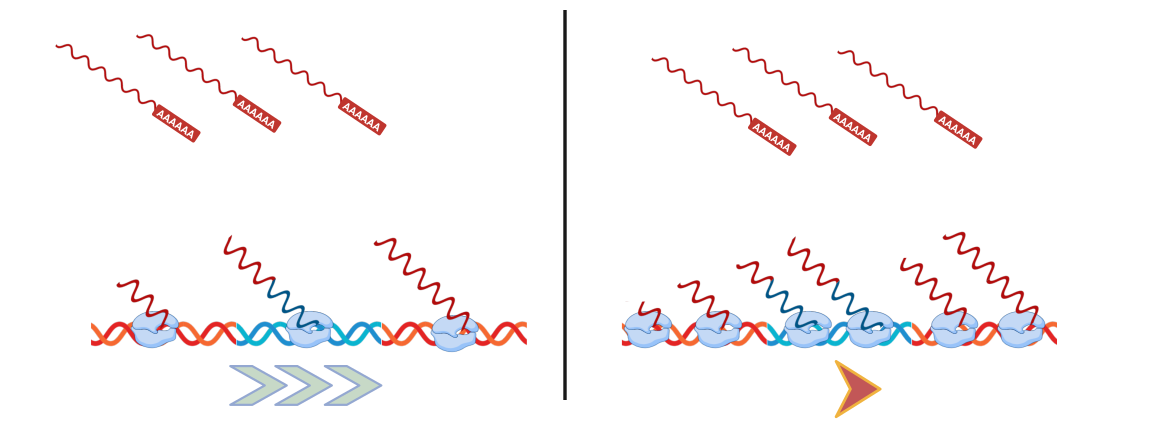
\includegraphics[scale=0.32]{pol_ii_speed.png}
		\end{center}
		
		\begin{itemize}			
			\item Slower speed $\implies$ higher occupancy of DNA by RNA polymerases $\implies$ more nascent RNA $\implies$ higher fraction of intronic reads.
						
	\end{itemize}	
	\end{frame}
	
	\begin{frame}
		\frametitle{C. elegans with mutation that slows Pol II }			
		\begin{center}
			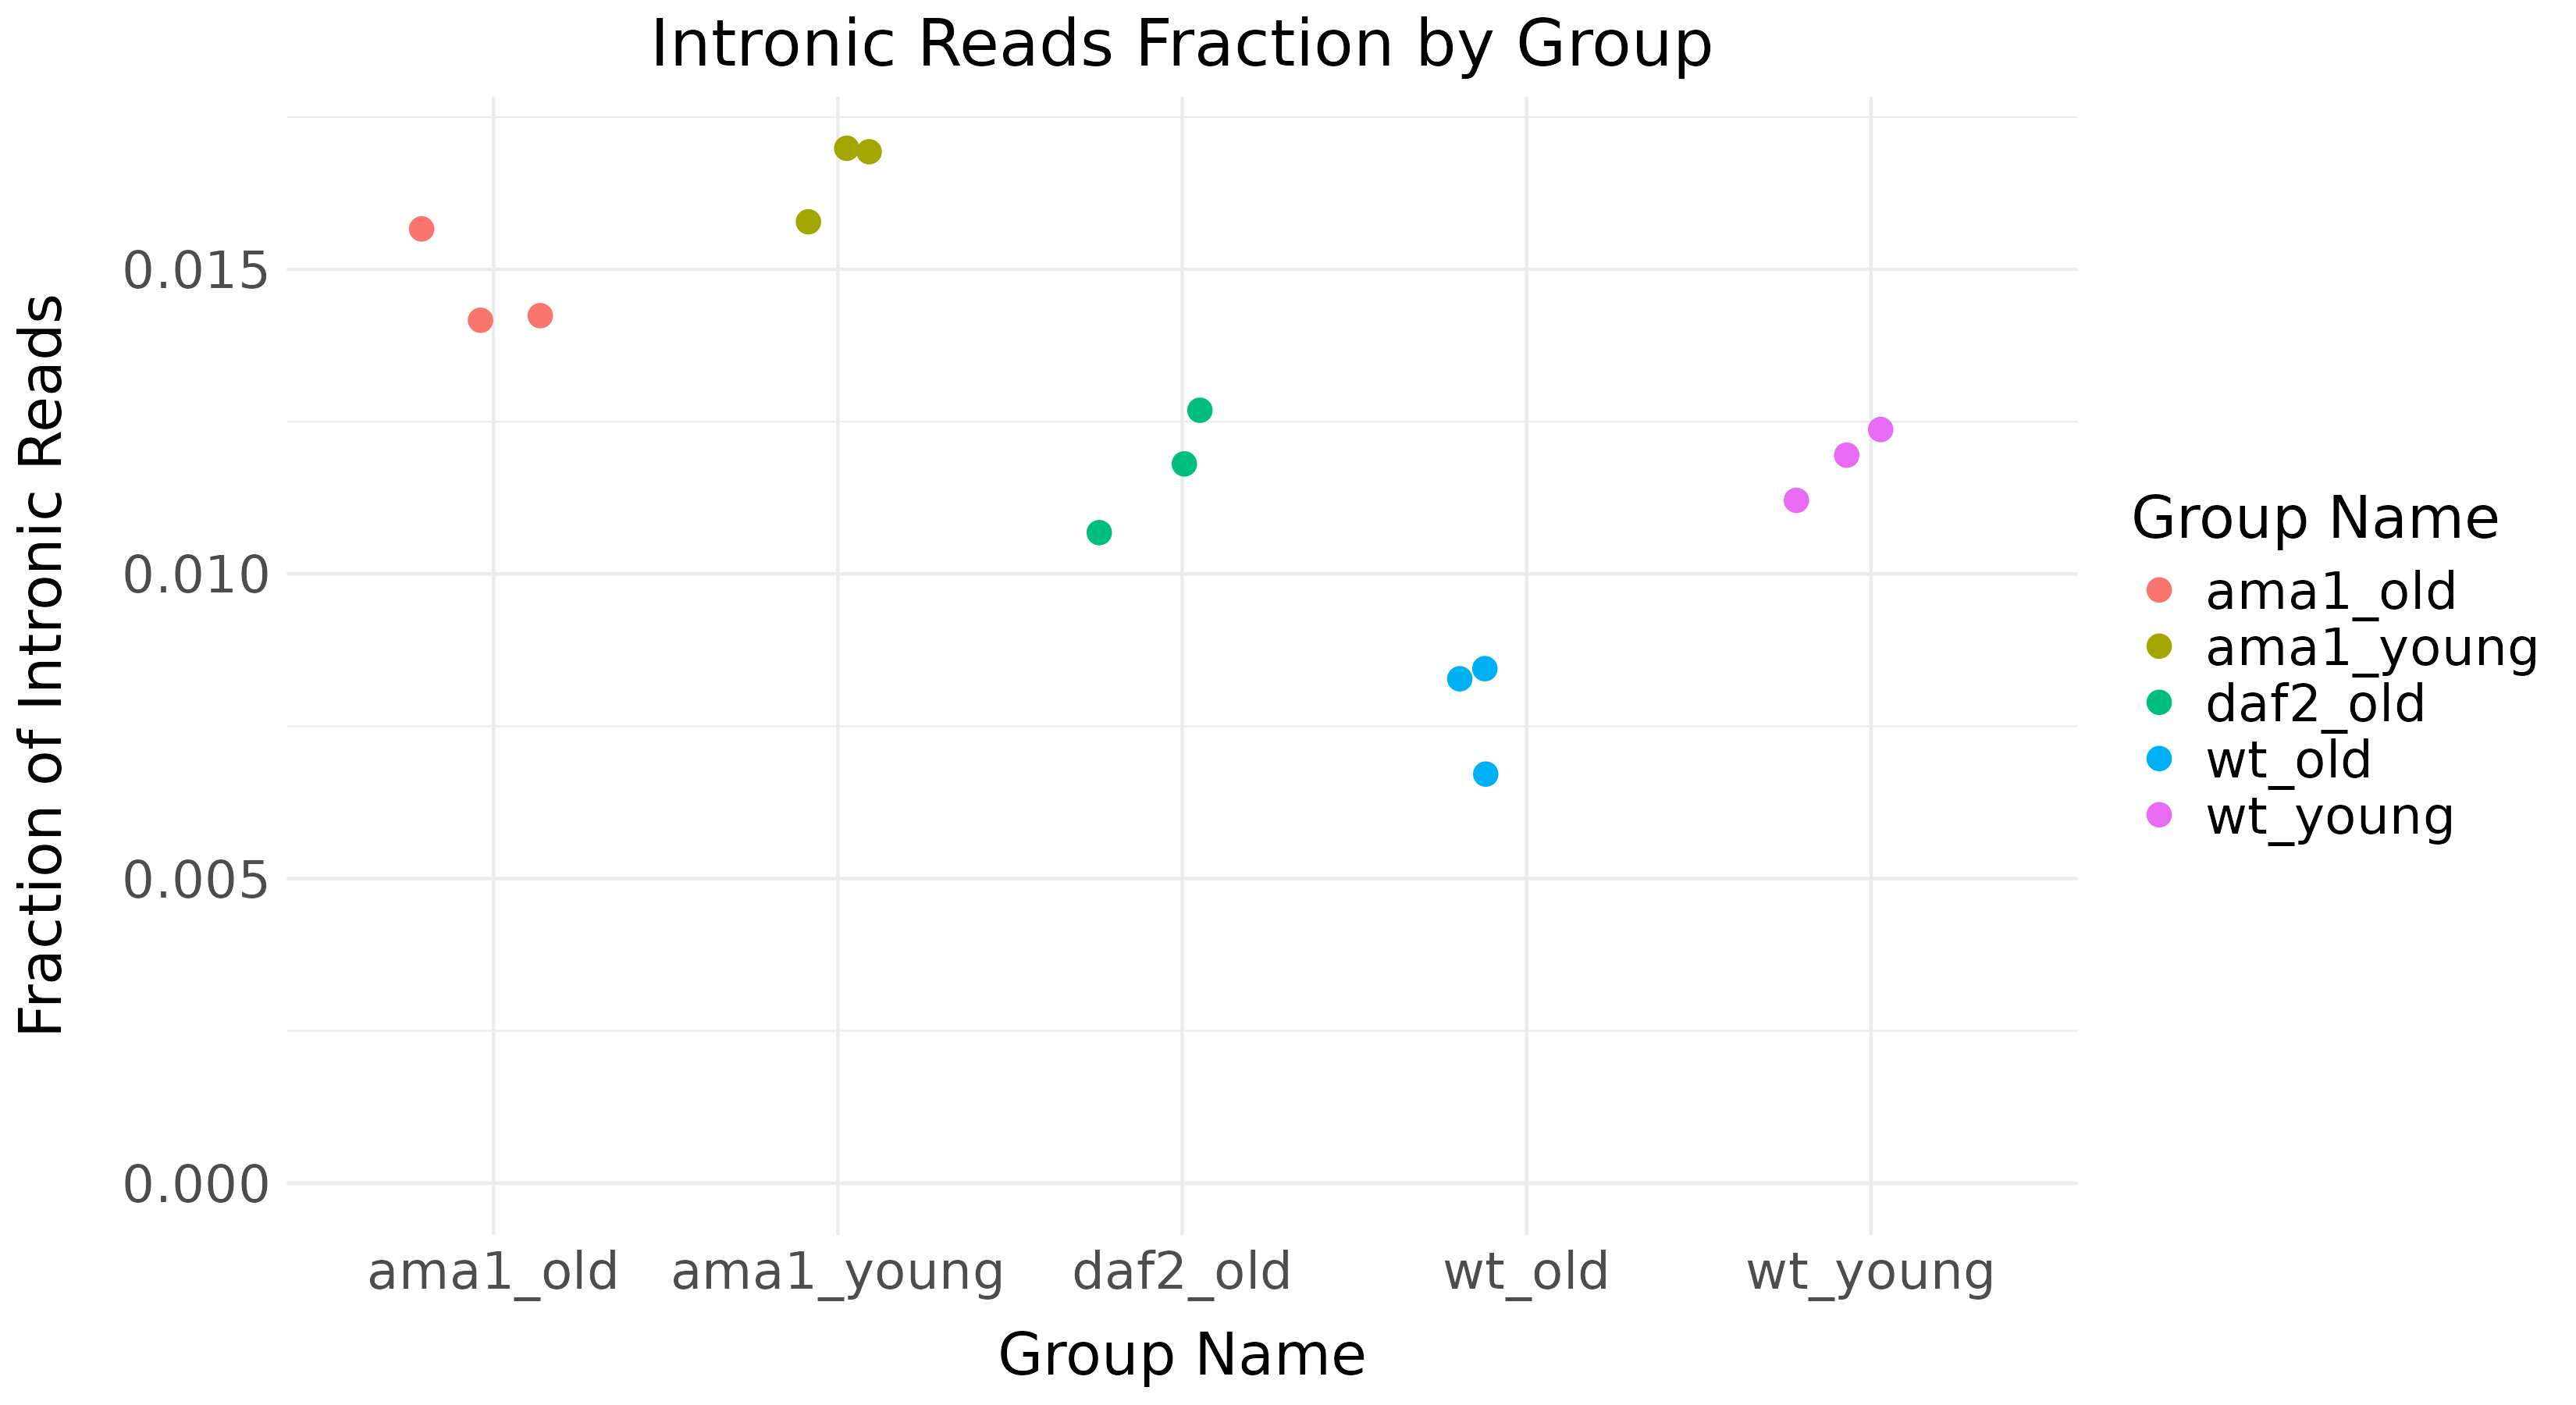
\includegraphics[scale=0.42]{intron_fraction.png}
		\end{center}
		\begin{itemize}
			\item Total RNA-seq samples of C. elegans with mutation decreasing RNA Pol II speed contain more intronic reads than wild-type control.    
			
		\end{itemize}
	\end{frame}
	
	
	
	
	\begin{frame}
		\frametitle{The End}
		Thank you for your attention!
		\begin{center}	
			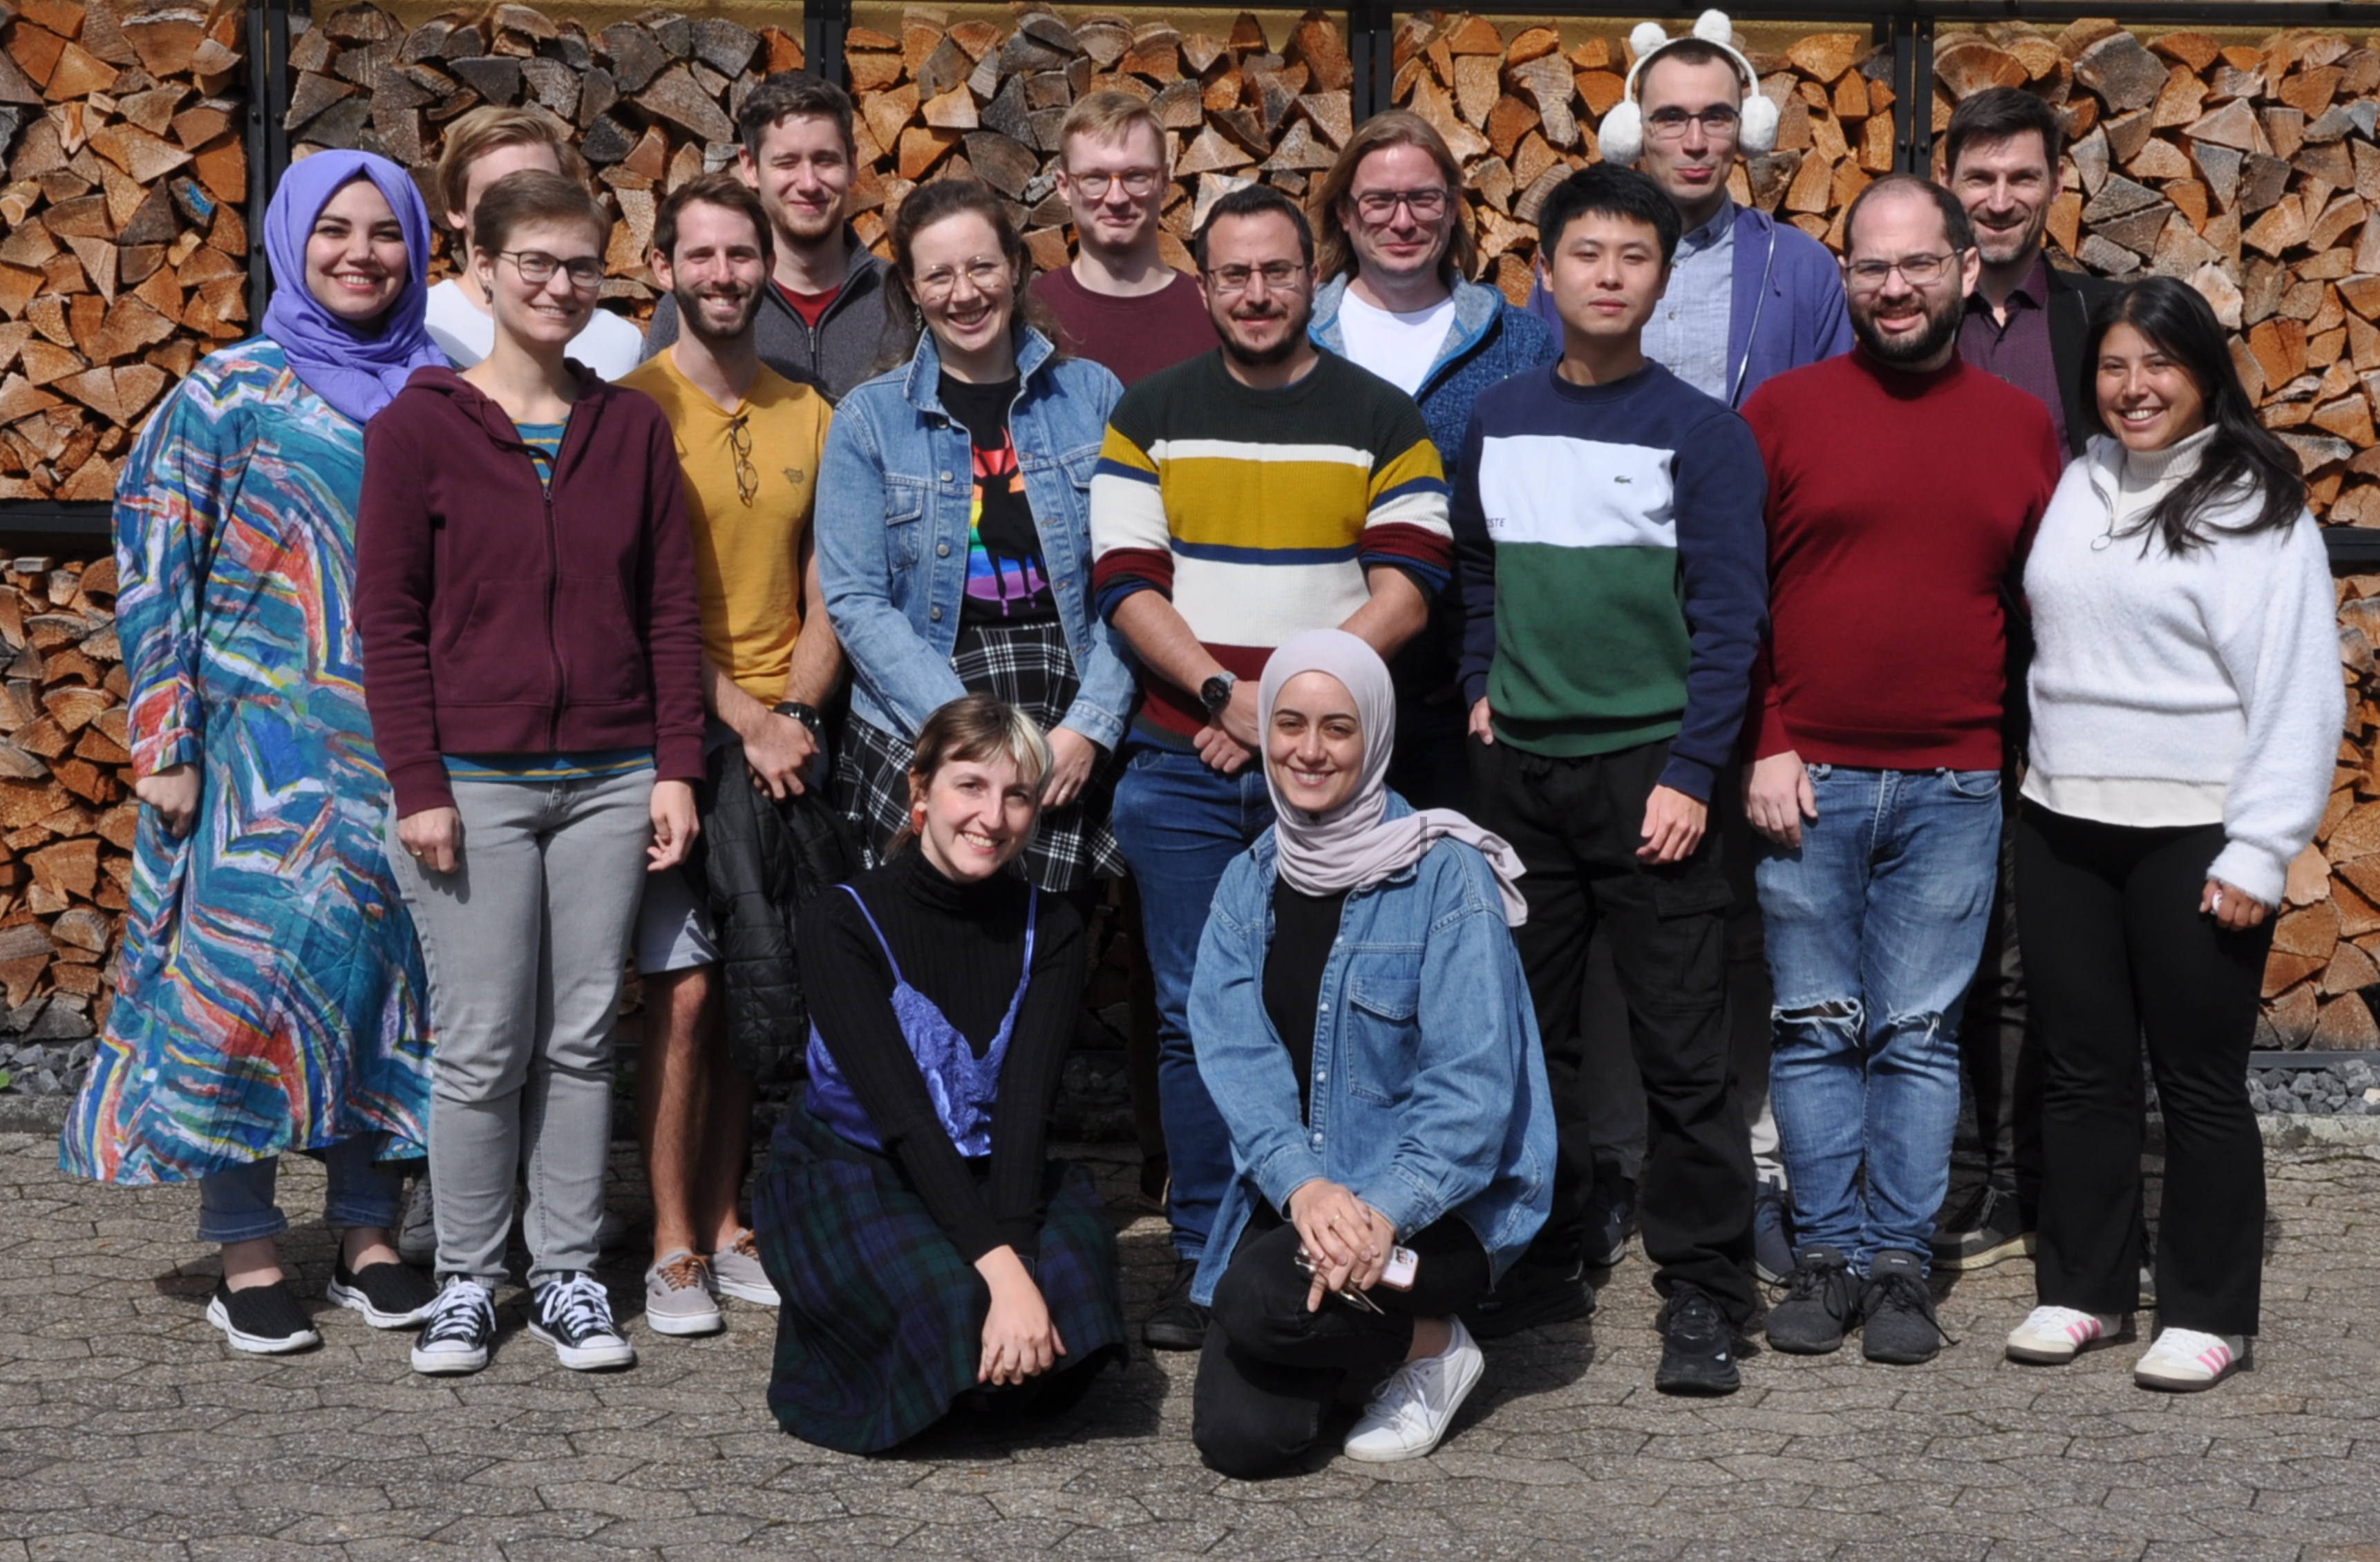
\includegraphics[scale=0.07]{group_picture.png}
		\end{center}
		
		\tiny{Illustrations and animations were created using BioRender and Manim.}
	\end{frame}
	
	
\end{document}
